
\documentclass[11pt]{article}
\usepackage[utf8]{inputenc}

\usepackage{comment}
\usepackage{amsmath}
\usepackage{amsfonts}
\usepackage{amsthm}
\usepackage{mathtools}
\usepackage{amssymb}
\usepackage{verbatim}
\usepackage[shortlabels]{enumitem}
\DeclarePairedDelimiter\ceil{\lceil}{\rceil}
\DeclarePairedDelimiter\floor{\lfloor}{\rfloor}



\newcommand{\bd}{\text{bd}}
\newcommand{\cl}{\text{cl}}
\newcommand{\inte} {\text{int}}

\newcommand{\cA}{ {\cal A} }
\newcommand{\fA}{ {\mathfrak{A}} }
\newcommand{\cB}{ {\cal B} }
\newcommand{\cD}{ {\cal D} }
\newcommand{\cF}{ {\cal F} }
\newcommand{\cL}{ {\cal L} }
\newcommand{\cM}{ {\cal M} }
\newcommand{\fM}{ {\mathfrak{M}} }
\newcommand{\cN}{ {\cal N} }
\newcommand{\cP}{ {\cal P} }
\newcommand{\cV}{ {\cal V} }
\newcommand{\cW}{ {\cal W} }

\newcommand{\bC}{ {\mathbb{C}} }
\newcommand{\bN}{ {\mathbb{N}} }
\newcommand{\bQ}{ {\mathbb{Q}} }
\newcommand{\bR}{ {\mathbb{R}} }
\newcommand{\bZ}{ {\mathbb{Z}} }

\newcommand{\ba}{ \vec{a} }
\newcommand{\bb}{ \vec{b} }
\newcommand{\ve}{ \vec{e} }
\newcommand{\pp}{ \vec{p} }
\newcommand{\qq}{ \vec{q} }
\newcommand{\ts}{ \vec{s} }
\newcommand{\uu}{ \vec{u} }
\newcommand{\vv}{ \vec{v} }
\newcommand{\ww}{ \vec{w} }
\newcommand{\xx}{ \vec{x} }
\newcommand{\yy}{ \vec{y} }
\newcommand{\zz}{ \vec{z} }
\newcommand{\zv}{ \vec{0} }

\newcommand{\aks}{ ( \, \ba_k \, )_{k=1}^{\infty} }
\newcommand{\xks}{ ( \, \xx_k \, )_{k=1}^{\infty} }
\newcommand{\yks}{ ( \, \yy_k \, )_{k=1}^{\infty} }
\newcommand{\qks}{ ( q_k )_{k=1}^{\infty} }
\newcommand{\tks}{ ( t_k )_{k=1}^{\infty} }

\newcommand{\limk}{ \lim_{k \to \infty} }
\newcommand{\ee}{ \varepsilon }


\setlength{\textwidth}{6in}
\setlength{\textheight}{8.75in}
\setlength{\oddsidemargin}{.3in}
\setlength{\topmargin}{-0.1in}
\setlength{\baselineskip}{14pt}

\pagestyle{headings}

\title{Fluorescence distributions in combinatorial models of amyloid fibrils composed of split-YFP, Sup35p, and CFP}
\author{Daniel Tianming Chen \\ \texttt{dchen0@pm.me}}
%\date{June 2017}

\usepackage[numbers]{natbib}
\usepackage{graphicx}
\usepackage{url}

\begin{document}

\maketitle

\begin{abstract}
We study four combinatorial models of fluorescence in amyloid fibrils---split-YFP alone, split-YFP with Sup35p, FRET YFP/CFP, and FRET YFP/CFP with Sup35p---and show that the expected fluorescence ratio---$R_{\text{SY}}(n) := 2E(n)/n$ for split-YFP systems, $R_{\text{F}}(n) := E(n)/n$ for FRET---converges to $2/3$, $1/3$, $1/2$, and $2/9$ respectively as the amyloid length $n \to \infty$. For split-YFP systems, we derive exact probability distributions $P(n,k)$ via generating functions applied to constrained binary strings, obtaining closed-form evaluations of $k \cdot 2^k$-weighted sums along the shallow diagonals of Pascal's triangle---identities related to known sequences (OEIS A127976, A095977) but arising here in a new biophysical context. These results are independently verified by Markov chain arguments. For FRET systems, the absence of a blocking constraint permits a direct linearity-of-expectation computation. All expected value formulas are exact for finite $n$, not merely asymptotic; the full distributions $P(n,k)$ are given in closed form for Sections 2 and 4, and via an explicit combinatorial formula (involving a convolution over compositions) for Sections 3 and 5.
\end{abstract}

\section{Introduction}
\textit{Amyloids} are fibrillar protein aggregates characterized by their distinctive $\beta$-sheet structure, where proteins self-assemble into highly ordered stacks \cite{chiti2006}. For the purposes of our mathematical analysis, we can abstract these complex biochemical structures into a simplified model where individual proteins, denoted as A,B,C,..., form sequential patterns in their stacking arrangements (e.g., ABBACCBCBCA...). This abstraction, while preserving the essential features of protein ordering within amyloid fibrils, transforms a complex biophysical system into a tractable mathematical framework. Our combinatorial approach follows the general framework of analytic combinatorics \cite[Ch.~I]{flajolet2009}. By viewing amyloid assembly through this lens, we can leverage classical combinatorial enumeration methods to analyze their structural properties, providing insights into both their formation patterns and potential biological implications. In particular, we study amyloids of different compositions, firstly just Split Yellow Fluorescent Proteins (split-YFP), a technique based on bimolecular fluorescence complementation \cite{hu2002}, then split-YFPs and Saccharomyces cerevisiae eukaryotic translation release factor Sup35p, and finally split-YFP and Sup35p under F\"{o}rster resonance energy transfer (FRET) \cite{forster1948} lighting. A specific quantity of interest is the expected number of fluorescing vertices, i.e., points between two proteins in the amyloid stack that fluoresce. We derive the full probability distributions $P(n,k)$ for the number of fluorescing sites and closed-form expressions for the expected values using combinatorial generating functions, Markov chains, and regular expressions. In the split-YFP settings, the adjacency blocking constraint leads to nontrivial combinatorial identities involving sums such as $\sum_{k \ge 1}^{\floor{n/2}} k\, 2^k \binom{n-k}{k}$, which we evaluate via generating function techniques \cite{wilf2006}. Two independent derivations---direct summation and Markov chain arguments---yield the same closed forms, providing mutual verification. The limiting fluorescence ratios are $2/3$, $1/3$, $1/2$, and $2/9$ for the four protein systems studied. The closed-form identities that arise turn out to match known OEIS sequences (A127976, A095977); the contribution of this work is not the identities themselves, but the combinatorial pipeline connecting a biophysical model to these sequences, providing a new interpretation in terms of fluorescence statistics. Several modeling assumptions should be stated at the outset. First, we assume that proteins are independently and uniformly distributed in the amyloid sequence. Real amyloid assembly is templated and cooperative \cite{chiti2006}, so this i.i.d.\ assumption constitutes a \textit{combinatorial null model}---a baseline against which non-random assembly effects could be detected, rather than a mechanistic description of fibril growth. Second, in the split-YFP sections, we model fluorophore reconstitution as a purely combinatorial adjacency event; we do not capture the irreversible, thermodynamically driven nature of bimolecular fluorescence complementation \cite{hu2002}. Third, in the FRET sections, we restrict interactions to nearest neighbors in the fibril. In practice, the inter-strand spacing in cross-$\beta$ amyloid structure is approximately 0.47\,nm, while the F\"{o}rster radius for the CFP--YFP pair is approximately 4.9\,nm \cite{forster1948, lakowicz2006}, so FRET can occur across roughly ten subunits. The nearest-neighbor restriction is therefore a significant simplification adopted for analytical tractability; extending the model to a larger interaction radius would change the combinatorial structure. Finally, the equal-concentration assumption ($p = 1/2$ or $1/3$ per protein type) is adopted throughout; we discuss the generalization to unequal concentrations in Section 6.

\section{Analysis of exclusively split-YFP Amyloids}
Let us first analyze amyloids consisting solely of YFP. YFP is a single polypeptide chain that can be split into two fragments, referred to as split-YFP. Call the distinct halves A and B. It is when these two halves A and B fuse that fluorescence occurs at the point of contact. There are no restrictions on the patterns in the amyloid - one can view all combinations of such halves via the regular expression $\{A,B\}^*$. 

We are interested in positions of an amyloid where A and B come together and fuse, producing yellow fluorescence. Such a scenario is essentially the reconstitution of the full fluorophore structure of YFP. We refer to such points in the amyloid stack as \textit{vertices} throughout this paper.

Let $n$ be the number of split-YFPs in a given amyloid. Clearly, there are $2^n$ possible amyloids of length $n$.

We will start with the case where the halves of Split-YFP are well-mixed in a neutral solution and of equal concentrations, and are thus equally likely to appear as the next protein in an amyloid sequence. 

\subsection{Lighting Patterns and 01 representations}

We abstract away from A and B specifically and instead analyze the ``lighting patterns'' of amyloids of length $n$, defined as follows.

We ask: How many distinct patterns of fluorescing locations could we possibly see from an amyloid of length n?

We define the \textit{01 representation} (or \textit{01 pattern}) of an amyloid $s_1 s_2 \cdots s_n \in \{A,B\}^n$ as the binary string $f_1 f_2 \cdots f_n \in \{0,1\}^n$ given by:
\[
f_i = \begin{cases}
0, & \text{if } i = 1, \\
1, & \text{if } i \ge 2,\ s_i \neq s_{i-1}, \text{ and } f_{i-1} = 0, \\
0, & \text{otherwise.}
\end{cases}
\]
Informally, $f_i = 1$ indicates that a fusion occurs between positions $i-1$ and $i$, attributed to the later index $i$: the protein $s_i$ differs from its neighbor $s_{i-1}$ and that neighbor was not already consumed by a prior fusion. The first protein always receives $f_1 = 0$ since there is no predecessor. The blocking constraint ($f_{i-1} = 0$ required) ensures that both proteins in a fused pair are ``used up,'' preventing cascading fusions. Note that the 01 representation has the same length as the amyloid, and the mapping $f$ is well-defined for any sequence in $\{A,B\}^n$.

The left-to-right, greedy pairing rule reflects the sequential nature of amyloid polymerization: proteins are incorporated one at a time at the growing end of the fibril, and each newly added protein either fuses with the current endpoint or does not. This greedy convention is motivated by the kinetics of sequential assembly---once a split-YFP pair reconstitutes, the resulting fluorophore is thermodynamically stable and irreversible \cite{hu2002}, so later arrivals cannot displace it. We note that on a path graph, the greedy matching (always fuse when possible) is in fact optimal: it yields the same count as a maximum matching of the completed static sequence. We prove this by induction on $n$. For $n \le 2$ the claim is trivial. For the inductive step, suppose the first fusible pair is at positions $(i, i+1)$. If we take it, the remaining sequence from position $i+2$ onward is handled optimally by the inductive hypothesis, yielding $1 + M(i+2, \ldots, n)$ fusions where $M$ denotes the maximum matching. If we skip it, the best we can achieve from position $i$ onward is $M(i, \ldots, n)$. But skipping $(i, i+1)$ frees $i+1$ only to potentially pair with $i+2$---yet $i+2$ can equally pair with $i+3$ regardless, so skipping gains at most zero net fusions. Hence taking the first available fusion is always optimal, and greedy equals maximum matching on paths. Thus the sequential and static interpretations of the model are equivalent.

For example, if we have ABBAAAAABA, then reading from left to right (because we have to think about how these proteins were added one at a time to analyze which ones fused), we get the 01 representation 0101000010. Writing these two representations side by side shows it:

\begin{alignat*}{10}
&A &B &B &A &A &A &A &A &B &A \\
&0 &1 &0 &1 &0 &0 &0 &0 &1 &0
\end{alignat*}


We always start with a 0, since the first protein cannot cause the (non-existent) previous protein to fluoresce. Doing this, we no longer need think about whether we started with an A or a B.

As another example,

\begin{alignat*}{34}
&B &B &B &B &A &B &A &B &A &B &A &B &A &B &A &B &A &B &A &A &A &A &B &A &A &B &A &B &B &B &B &A &B &A  \\
&0 &0 &0 &0 &1 &0 &1 &0 &1 &0 &1 &0 &1 &0 &1 &0 &1 &0 &1  &0 &0 &0 &1 &0 &0 &1 &0 &1 &0 &0 &0 &1 &0 &1
\end{alignat*} 
We observe that an unambiguous regular expression for these 01 patterns is $(0^*01)^* 0^*$ (non-ambiguous in the sense required by the symbolic method: each string has a unique parse). Note that if we were looking at an amyloid without knowing what the proteins actually were, we would still be able to identify its 01 pattern by looking at the fluorescing locations. Indeed, each fluorescing location corresponds to a 1.

We can count the total number of distinct 01 patterns of length $n$ using the symbolic method for regular expressions \cite[\S I.4]{flajolet2009}. Note that $(0^*01)^* 0^* = (0^+1)^* 0^*$: each block $0^*01$ consists of zero or more leading zeros followed by $01$, so the trailing $0$ of $0^*$ and the leading $0$ of $01$ merge to give at least one zero before the $1$, hence $0^*01 = 0^+1$. We assign weight $x$ per symbol. Each block $0^*01 = 0^+1$ has generating function $\frac{x}{1-x} \cdot x = \frac{x^2}{1-x}$, and the Kleene star $(0^*01)^*$ has generating function $\frac{1}{1 - x^2/(1-x)} = \frac{1-x}{1-x-x^2}$. Including the trailing $0^*$ with generating function $\frac{1}{1-x}$, we obtain:
\[
G(x) := \sum_{n=0}^\infty a_n x^n = \frac{1-x}{1-x-x^2} \cdot \frac{1}{1-x} = \frac{1}{1-x-x^2}
\]

Since $(1-x-x^2)\sum_{n \ge 0} a_n x^n = 1$, we read off the recurrence $a_n = a_{n-1} + a_{n-2}$ for $n \ge 2$, with $a_0 = a_1 = 1$.

We see that $a_0 = 1$, $a_1 = 1$, $a_2 = 2$, $a_3 = 3$, $a_4 = 5$, $a_5 = 8$, etc.

So $a_n = F_{n+1}$, where $F_n$ is the Fibonacci sequence with the standard convention $F_1 = F_2 = 1$. The coefficients $\binom{n-k}{k}$ appearing in this sum are precisely the entries along the \textit{shallow diagonals} of Pascal's triangle, and the identity $a_n = F_{n+1}$ is a well-known consequence of summing along these diagonals. The weighted sums $S_1(n)$ and $S_2(n)$ evaluated in Section 2.4 can be viewed as weighted sums along these same diagonals, with each entry scaled by $k \cdot 2^k$.

\subsection{Probability of $k$ fluorescing vertices in length $n$ amyloid }

We now analyze the probability of seeing $k$ fluorescing vertices in an amyloid of length $n$.

%This is equivalent to the probability of observing an amyloid of length $n$ with $k$ 1's in its 01 pattern.

\subsubsection{Distinct 01 patterns with $k$ 1s}
First, let us count the number of 01 patterns of length $n$ with $k$ 1s. Our invariant states that no 1s may be adjacent, and the first digit must be a zero. Since $f_1 = 0$ always, the $k$ ones must be placed among positions $2, 3, \ldots, n$ (i.e., $n - 1$ available positions) with no two adjacent. This is equivalent to placing $k$ non-adjacent objects in $n - 1$ boxes, giving:
\[
N(n,k) := \binom{n-k}{k}, \quad k \leq \floor{n/2}
\]
Indeed, the number of ways to place $k$ non-adjacent objects in $m$ boxes is $\binom{m-k+1}{k}$ (see \cite[Exercise~1.34]{stanley2012}); setting $m = n - 1$ gives $\binom{n-k}{k}$ as claimed.


\subsubsection{Distinct amyloids with $k$ 1s}
Now, the number of distinct amyloids of length $n$ with $k$ fluorescing pairs is:
\[
    \cA(n,k) = 2^k \cdot N(n-2,k-1) + 2^{k+1}  \cdot N(n-1,k) = 2^k \binom{n-k-1}{k-1} + 2^{k+1} \binom{n-k-1}{k}
\]

To see this, we have two cases, where we fix $k = 5$ for the sake of example: 

\textbf{01 pattern ends with a 0}

Consider the following pattern. We write the number of possible proteins (A or B) at that location below the corresponding location of the pattern.
\begin{align*} 
    & 000010000101001000010000 \\
    & 211112111121211211112111
\end{align*}
Indeed, for each block of 0's, at the beginning of the block, any of either A or B may appear there, since it will not fuse with the previous protein. Then thereafter each protein is uniquely determined by this choice through to the 1 that appears.

Any pattern of this case therefore has $2^{k+1}$ possible amyloids associated with it. There are $N(n-1,k)$ possible patterns for this case. 

\textbf{01 pattern ends with a 1}

Consider the following 01 pattern. We write the number of possible proteins (A or B) at that location below the corresponding location of the 01 pattern.
\begin{align*} 
    & 000010000101001000000001 \\
    & 211112111121211211111111
\end{align*}

As we can see, putting a 1 at the end of the 01 pattern implies only $2^k$ possible amyloids with the particular pattern. There are $N(n-2, k - 1)$ patterns with this property.

\textbf{Verification.} For $n = 4$, $k = 1$: $\cA(4,1) = 2^1 \binom{2}{0} + 2^2 \binom{2}{1} = 2 + 8 = 10$. For $k = 2$: $\cA(4,2) = 2^2 \binom{1}{1} + 2^3 \binom{1}{2} = 4 + 0 = 4$ (the only 01 pattern is $0101$, giving amyloids ABAB, BABA, ABBA, BAAB). With $\cA(4,0) = 2$ (AAAA and BBBB), we have $2 + 10 + 4 = 16 = 2^4$. $\checkmark$

Hence the probability of seeing $k$ fluorescing pairs in an amyloid of length $n$ is

\[
P(n,k) = \frac{\cA(n,k)}{2^n}
\]

% \subsection{Probability of at least $m$ fluorescing locations}

% The probability of seeing at least $m$ fluorescing pairs on an amyloid of length $n$ is simply the sum:
% \[
%   P_{\geq}(n,m) = \frac{1}{2^n}\sum_{k = m}^{\floor{n/2}} \cA(n,k)
% \]
% since the events $k = m, \dots,  \floor{n/2}$ are independent.

\subsection{Expected number of fluorescing locations}

This is simply the sum:

\[
    E(n) = \frac{1}{2^n}\sum_{k \ge 1}^{\floor{n/2}} k \cdot \cA(n,k) = \frac{1}{2^n}\sum_{k \ge 1}^{\floor{n/2}} k \left( 2^k \binom{n-k-1}{k-1} + 2^{k+1} \binom{n-k-1}{k} \right)
\]

by definition of expected value.

\subsection{Expected percentage of proteins involved in fluorescence}

Since each fluorescing vertex involves two proteins, the fraction of proteins participating in fluorescence is:

\[
    R_{\text{SY}}(n) := \frac{2E(n)}{n} = \frac{1}{n \cdot 2^{n-1}}\sum_{k \ge 1}^{\floor{n/2}} k \left( 2^k \binom{n-k-1}{k-1} + 2^{k+1} \binom{n-k-1}{k} \right)
\]

We claim that
\begin{equation}\label{eq:sum1}
\sum_{k \ge 1}^{\floor{n/2}} k 2^k \binom{n-k-1}{k-1} = \frac{2^n (3n+2) + 2(6n-1)(-1)^n}{27}
\end{equation}

and

\begin{equation}\label{eq:sum2}
\sum_{k \ge 1}^{\floor{n/2}} k 2^k \binom{n-k-1}{k} = \frac{2^n (3n-4)-2(3n-2)(-1)^n}{27}
\end{equation}

We prove both identities using ordinary generating functions.

We will use the identity (see, e.g., \cite[\S 1.2]{wilf2006}) that for any fixed $j \ge 0$,
\begin{equation}\label{eq:binom-ogf}
\sum_{n \ge 2j} \binom{n-j}{j} x^n = \frac{x^{2j}}{(1-x)^{j+1}}
\end{equation}
which follows from the substitution $m = n - j$ and the known generating function $\sum_{m \ge j} \binom{m}{j} x^m = x^j/(1-x)^{j+1}$.

\textbf{Proof of (\ref{eq:sum1}).} Let $S_1(n) := \sum_{k \ge 1}^{\floor{n/2}} k\, 2^k \binom{n-k-1}{k-1}$. We derive the ordinary generating function $G_1(x) = \sum_{n \ge 0} S_1(n) x^n$.

Using the substitution $j = k - 1$,
\[
S_1(n) = \sum_{j \ge 0} (j+1)\, 2^{j+1} \binom{n - j - 2}{j}
\]
Since all terms are non-negative for $x > 0$, we may interchange the order of summation. Applying (\ref{eq:binom-ogf}) with a shift $n \mapsto n - 2$:
\[
G_1(x) = \sum_{j \ge 0}(j+1)\, 2^{j+1} \cdot \frac{x^{2j+2}}{(1-x)^{j+1}}
= \frac{2x^2}{1-x} \sum_{j \ge 0} (j+1) \left( \frac{2x^2}{1-x} \right)^j
\]
Setting $u = 2x^2/(1-x)$ and using $\sum_{j \ge 0}(j+1) u^j = 1/(1-u)^2$, we have
\[
G_1(x) = \frac{2x^2}{1-x} \cdot \frac{1}{(1-u)^2}
\]
Since $1 - u = (1 - x - 2x^2)/(1-x) = (1-2x)(1+x)/(1-x)$, this simplifies to
\[
G_1(x) = \frac{2x^2(1-x)}{(1-2x)^2(1+x)^2}
\]
We now perform a partial fraction decomposition:
\[
G_1(x) = \frac{\alpha}{1-2x} + \frac{\beta}{(1-2x)^2} + \frac{\gamma}{1+x} + \frac{\delta}{(1+x)^2}
\]
Multiplying both sides by $(1-2x)^2(1+x)^2$ and evaluating at $x = 1/2$ gives $\beta = 1/9$, and at $x = -1$ gives $\delta = 4/9$. Expanding the right-hand side and comparing coefficients of $x^0$ and $x^1$ then yields $\alpha = -1/27$ and $\gamma = -14/27$. Now, using the standard power series
\begin{align*}
\frac{1}{1-2x} &= \sum_{n \ge 0} 2^n x^n, &
\frac{1}{(1-2x)^2} &= \sum_{n \ge 0} (n+1)\, 2^n x^n \\
\frac{1}{1+x} &= \sum_{n \ge 0} (-1)^n x^n, &
\frac{1}{(1+x)^2} &= \sum_{n \ge 0} (n+1)(-1)^n x^n
\end{align*}
we extract the coefficient of $x^n$:
\begin{align*}
S_1(n) &= -\frac{1}{27} \cdot 2^n + \frac{1}{9}(n+1)\, 2^n - \frac{14}{27}(-1)^n + \frac{4}{9}(n+1)(-1)^n \\
&= \frac{1}{27}\left[ 2^n(-1 + 3n + 3) + (-1)^n(-14 + 12n + 12) \right] \\
&= \frac{2^n(3n+2) + 2(6n-1)(-1)^n}{27}
\end{align*}
as claimed. $\square$

\textbf{Proof of (\ref{eq:sum2}).} Let $S_2(n) := \sum_{k \ge 1}^{\floor{n/2}} k\, 2^k \binom{n-k-1}{k}$. As before, applying (\ref{eq:binom-ogf}):
\[
G_2(x) = \sum_{n \ge 0} S_2(n) x^n = \sum_{k \ge 1} k \cdot 2^k \cdot \frac{x^{2k+1}}{(1-x)^{k+1}} = \frac{x}{1-x} \cdot \frac{u}{(1-u)^2}
\]
where $u = 2x^2/(1-x)$ as before. This simplifies to
\[
G_2(x) = \frac{2x^3}{(1-2x)^2(1+x)^2}
\]
Performing partial fractions, evaluating at $x = 1/2$ gives $\beta = 1/9$ and at $x = -1$ gives $\delta = -2/9$. Comparing coefficients of $x^0$ and $x^1$ yields $\alpha = -7/27$ and $\gamma = 10/27$. Extracting coefficients:
\begin{align*}
S_2(n) &= -\frac{7}{27}\cdot 2^n + \frac{1}{9}(n+1)\,2^n + \frac{10}{27}(-1)^n - \frac{2}{9}(n+1)(-1)^n \\
&= \frac{1}{27}\left[2^n(-7+3n+3) + (-1)^n(10-6n-6)\right] \\
&= \frac{2^n(3n-4) - 2(3n-2)(-1)^n}{27}
\end{align*}
as claimed. $\square$

Substituting (\ref{eq:sum1}) and (\ref{eq:sum2}):

\begin{align}
 R_{\text{SY}}(n) &= \frac{1}{n \cdot 2^{n-1}}\sum_{k \ge 1}^{\floor{n/2}} k \left( 2^k \binom{n-k-1}{k-1} + 2^{k+1} \binom{n-k-1}{k} \right) \\
 &= \frac{1}{n \cdot 2^{n-1}} \left(\frac{2^n (3n+2) + 2(6n-1)(-1)^n}{27}  + 2 \cdot \frac{2^n (3n-4)-2(3n-2)(-1)^n}{27} \right) \\
 &= \frac{1}{n \cdot 2^{n-1}} \cdot \frac{2^n(9n-6) + 6(-1)^n}{27} \\
 &= \frac{2(9n-6)}{27n} + \frac{6(-1)^n}{27n \cdot 2^{n-1}} \\
 &= \frac{2(3n-2)}{9n} + \frac{2(-1)^n}{9n \cdot 2^{n-1}}
\end{align}

Then as $n \rightarrow \infty$, the second term vanishes and we have

\begin{align}
    \lim_{n \rightarrow \infty} R_{\text{SY}}(n) &= \lim_{n \rightarrow \infty} \frac{2(3n-2)}{9n} = \frac{6}{9} = \frac{2}{3}
\end{align}

\subsubsection{Weighted shallow diagonal identities}

The identities (\ref{eq:sum1}) and (\ref{eq:sum2}) have a natural interpretation in terms of Pascal's triangle. Recall that the entries along the shallow diagonals of Pascal's triangle are $\binom{n-k}{k}$ for $k = 0, 1, \ldots, \floor{n/2}$, and their sum $\sum_{k=0}^{\floor{n/2}} \binom{n-k}{k} = F_{n+1}$ yields the Fibonacci numbers (Section 2.1). The identities (\ref{eq:sum1}) and (\ref{eq:sum2}) provide closed-form evaluations of \textit{weighted} sums along these same diagonals, where each entry is scaled by $k \cdot 2^k$:
\begin{align}
\sum_{k=1}^{\floor{n/2}} k \cdot 2^k \binom{n-k-1}{k-1} &= \frac{2^n(3n+2) + 2(6n-1)(-1)^n}{27} \label{eq:diag1} \\[6pt]
\sum_{k=1}^{\floor{n/2}} k \cdot 2^k \binom{n-k-1}{k} &= \frac{2^n(3n-4) - 2(3n-2)(-1)^n}{27} \label{eq:diag2}
\end{align}
These identities arise here from the fluorescence analysis, but the sequences themselves are not new. Specifically, $S_1(n) = 2 \cdot \text{A127976}(n-1)$ and $S_2(n) = \text{A095977}(n-2)$, where A127976 arises as a convolution of Jacobsthal numbers and A095977 counts $2 \times 2$ tiles in tilings of $3 \times (n+1)$ rectangles. Both sequences satisfy the linear recurrence $a_n = 2a_{n-1} + 3a_{n-2} - 4a_{n-3} - 4a_{n-4}$ with different initial conditions, which can be verified from the generating function denominator $(1+x)^2(1-2x)^2 = 1 - 2x - 3x^2 + 4x^3 + 4x^4$. Direct computation confirms: $S_1(2) = 2 = 2 \cdot \text{A127976}(1)$ and $S_2(3) = 2 = \text{A095977}(1)$, with subsequent values matching by the shared recurrence.

The fact that the same sequences govern such disparate problems---protein fluorescence in amyloid fibrils, convolutions of Jacobsthal numbers, and rectangle tilings---reflects a deeper structural phenomenon: all three settings reduce to constrained binary strings enumerated by the same rational generating functions with denominator $(1+x)^2(1-2x)^2$. The contribution of the present work is not the identities themselves, but the combinatorial pipeline that connects the biophysical model (protein sequences $\to$ constrained 01 patterns $\to$ generating functions) to these known sequences, providing a new interpretation in terms of fluorescence statistics.

As a corollary, the linear combination $S_1(n) + 2\,S_2(n) = \bigl[2^n(9n-6) + 6(-1)^n\bigr]/27$ governs the expected fluorescence in split-YFP amyloids, connecting these combinatorial identities directly to the biophysical application.

\subsubsection{Alternative derivation via Markov chain}

We can also derive $E(n)$ directly by a Markov chain argument \cite{norris1997}, bypassing $\cA(n,k)$ entirely. Consider building an amyloid one protein at a time, where each protein is independently A or B with equal probability $1/2$. Define two states based on the rightmost protein:
\begin{itemize}
\item \textbf{State $p$}: the rightmost protein is \textit{not} part of a fused pair.
\item \textbf{State $q$}: the rightmost protein is part of a fused pair.
\end{itemize}

From state $p$ (say the rightmost protein is A, unfused): with probability $1/2$ the next protein is A (same type, no fusion, stay in $p$), and with probability $1/2$ it is B (fusion, go to $q$, $+1$ fluorescence). By symmetry, the case for B is identical. So from $p$: transition to $p$ with probability $1/2$ and to $q$ with probability $1/2$, with expected fluorescence $1/2$.

From state $q$ (rightmost protein is fused): the next protein is A or B each with probability $1/2$, and in either case goes to state $p$ with no fluorescence (since the current protein is already fused). So from $q$: transition to $p$ with probability $1$.

With $p_1 = 1$ (the first protein is always unfused), the recurrence is
\[
p_{n+1} = \underbrace{\tfrac{1}{2}\, p_n}_{\text{stay in }p} + \underbrace{(1 - p_n)}_{\text{from }q\text{ to }p} = 1 - \tfrac{1}{2}\, p_n
\]
which has fixed point $p^* = 2/3$ and general solution
\[
p_n = \frac{2}{3} + \frac{1}{3}\left(-\frac{1}{2}\right)^{n-1}
\]

The expected fluorescence contributed by the $(n+1)$th protein is $e_{n+1} = \frac{1}{2} p_n$, so
\begin{align*}
E(n) = \sum_{i=2}^{n} e_i &= \frac{1}{2} \sum_{j=1}^{n-1} p_j = \frac{1}{2} \sum_{j=1}^{n-1} \left[ \frac{2}{3} + \frac{1}{3}\left(-\frac{1}{2}\right)^{j-1} \right] \\
&= \frac{n-1}{3} + \frac{1}{6} \cdot \frac{1 - (-1/2)^{n-1}}{3/2} = \frac{n-1}{3} + \frac{1}{9}\left(1 - \left(-\frac{1}{2}\right)^{n-1}\right)
\end{align*}

Therefore
\[
R_{\text{SY}}(n) = \frac{2E(n)}{n} = \frac{2(n-1)}{3n} + \frac{2}{9n}\left(1 - \left(-\frac{1}{2}\right)^{n-1}\right) \longrightarrow \frac{2}{3} \text{ as } n \to \infty
\]

Since this must agree with the combinatorial derivation, equating the two expressions for $E(n)$ provides an independent verification of the sum identities (\ref{eq:sum1}) and (\ref{eq:sum2}). Specifically,
\[
\frac{S_1(n) + 2\,S_2(n)}{2^n} = \frac{n-1}{3} + \frac{1}{9}\left(1 - \left(-\frac{1}{2}\right)^{n-1}\right)
\]
To verify this, substitute the closed forms from (\ref{eq:sum1}) and (\ref{eq:sum2}):
\[
\frac{S_1(n) + 2S_2(n)}{2^n} = \frac{2^n(9n-6) + 6(-1)^n}{27 \cdot 2^n} = \frac{3n-2}{9} + \frac{2(-1)^n}{9 \cdot 2^n}
\]
while the Markov chain gives $E(n) = \frac{n-1}{3} + \frac{1}{9} - \frac{(-1)^{n-1}}{9 \cdot 2^{n-1}} = \frac{3n-2}{9} + \frac{2(-1)^n}{9 \cdot 2^n}$, confirming the two expressions are identical.

We can also verify the above via computer simulation (see \texttt{split\_yfp\_simulation.py}; all scripts are available at \url{https://github.com/danielchen0/amyloids}). A sample of computed values is shown in Table~\ref{tab:splityfp}, and the first 400 values appear in Figure~\ref{fig:splityfp}.

\begin{table}[ht]
\centering
\begin{tabular}{rc|rc|rc}
\hline
$n$ & $R_{\text{SY}}(n)$ & $n$ & $R_{\text{SY}}(n)$ & $n$ & $R_{\text{SY}}(n)$ \\
\hline
2 & 0.500000 & 10 & 0.622266 & 20 & 0.644444 \\
3 & 0.500000 & 11 & 0.626243 & 25 & 0.648889 \\
4 & 0.562500 & 12 & 0.629639 & 50 & 0.657778 \\
5 & 0.575000 & 13 & 0.632474 & 100 & 0.662222 \\
6 & 0.593750 & 14 & 0.634923 & 200 & 0.664444 \\
7 & 0.602679 & 15 & 0.637036 & 400 & 0.665556 \\
\hline
\multicolumn{6}{c}{$R_{\text{SY}}(n) \to 2/3 \approx 0.666667$} \\
\end{tabular}
\caption{Sample values of $R_{\text{SY}}(n)$ for split-YFP amyloids.}
\label{tab:splityfp}
\end{table}

\begin{figure}[ht]
\centering
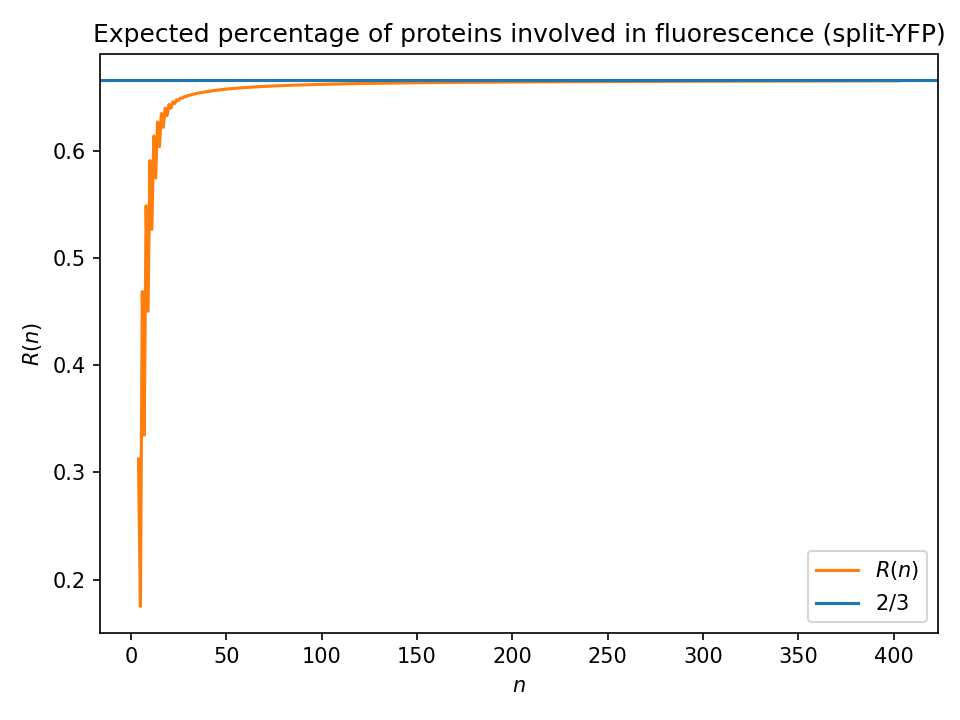
\includegraphics[width=0.75\textwidth]{SplitYFPamyloids.png}
\caption{$R_{\text{SY}}(n)$ for split-YFP amyloids. The blue line is $2/3$ and the orange curve is the exact $R_{\text{SY}}(n)$. The exponential correction term $O((1/2)^n/n)$ yields rapid convergence.}
\label{fig:splityfp}
\end{figure}


\section{Introducing Sup35p into Amyloids}
We now want to consider the facts above but with the introduction of yeast prion protein Sup35p (which we label with an $S$) into our amyloids. In our model, Sup35p is treated as completely inert: it cannot participate in any fluorescent interaction, and its sole effect is to sterically separate adjacent split-YFP halves, preventing them from conjoining and fluorescing. Our amyloids can now be described using the regular expression $\{A,B,S\}^*$. We would like to first analyze the case where Sup35p and the halves of Split-YFP come in equal concentrations, and are thus equally likely to occur as the next protein in an amyloid sequence.

\subsection{Number of distinct lighting patterns and 01 representations}
The introduction of Sup35p does not change this. When we abstract away the details we are still looking at 01 patterns of the form $(0^*01)^* 0^*$. Hence we have $F_{n+1}$ distinct lighting patterns for an amyloid of length $n$ (using the convention $F_1 = F_2 = 1$).

\subsection{Probability of $k$ fluorescing locations in length $n$ amyloid}

The key idea is that each 01 pattern with $k$ ones decomposes into $k$ ``active blocks'' of the form $0^+1$ (each containing exactly one fluorescing site), followed by a trailing run of zeros. The $k$ fluorescing sites partition the amyloid into these independent blocks, and the total count is obtained by summing over all ways to distribute the $n$ positions among the blocks and the tail, weighting each by the number of A-B-S protein patterns it admits.

Formally, the number of amyloids of length $n$ with $k$ fluorescing locations is:
\[
\cA(n,k) = \sum_{q=0}^{n - 2k} b_q \sum_{\substack{\sum_{i=1}^k \phi_i = n-q \\ \phi_i \ge 2}} \prod_{i=1}^k a_{\phi_i}
\]

The inner sum is a convolution over compositions of $n - q$ into $k$ parts, each of size $\ge 2$.

Here $a_0 = a_1 = 0, a_2 = 2$, $a_i = 2a_{i-1} + a_{i-2}, i > 2$
and $b_0 = 1, b_1 = 3$, $b_i = 2b_{i-1} + b_{i-2}, i > 1$.

Explicitly,

\[
b_n = - \frac{1}{2 + 2\sqrt{2}} \cdot \left(\frac{1}{-1-\sqrt{2}}\right)^n - \frac{1}{2-2\sqrt{2}} \cdot \left( \frac{1}{-1 +\sqrt{2}} \right)^n, n \ge 0 
\]

and

\[a_n = 
\begin{cases}
      0, & \text{if}\ n=0 \\
        \frac{3+2\sqrt{2}}{\sqrt{2}+2} \left( \frac{1}{-1-\sqrt{2}}\right)^n - \frac{3 - 2\sqrt{2} }{\sqrt{2}-2}\left( \frac{1}{-1 + \sqrt{2}} \right)^n  , & \text{if} \ n \geq 1
    \end{cases}
\]


And so the probability of $k$ fluorescing locations in an amyloid of length $n$ is $\cA(n,k)/3^n$.

\textbf{Worked example.} Consider $n = 4$, $k = 1$. A 01 pattern of length 4 with exactly one 1 decomposes as one block of the form $0^+1$ (of length $\phi_1$) followed by a tail of zeros (of length $q$), where $\phi_1 + q = 4$ and $\phi_1 \ge 2$. Using the recurrences, $a_2 = 2$, $a_3 = 4$, $a_4 = 10$, and $b_0 = 1$, $b_1 = 3$, $b_2 = 7$. The decomposition gives:
\begin{center}
\begin{tabular}{cccc}
$\phi_1$ & $q$ & 01 pattern & $a_{\phi_1} \cdot b_q$ \\
\hline
2 & 2 & 0100 & $2 \cdot 7 = 14$ \\
3 & 1 & 0010 & $4 \cdot 3 = 12$ \\
4 & 0 & 0001 & $10 \cdot 1 = 10$ \\
\end{tabular}
\end{center}
So $\cA(4,1) = 14 + 12 + 10 = 36$. One can verify by brute-force enumeration over all $3^4 = 81$ amyloids of length 4 that exactly 36 have precisely 1 fluorescing location.

The derivation of this formula proceeds by establishing a bijection between amyloids of length $n$ with $k$ fluorescing locations and tuples $(q, \phi_1, \ldots, \phi_k)$ specifying a block decomposition. Every 01 pattern with exactly $k$ ones has the form
\[
\underbrace{0\cdots 0\, 1}_{\phi_1} \; \underbrace{0\cdots 0\, 1}_{\phi_2} \; \cdots \; \underbrace{0\cdots 0\, 1}_{\phi_k} \; \underbrace{0\cdots 0}_{q}
\]
where $\phi_i \ge 2$ (each active block has at least one leading zero before its $1$) and $q \ge 0$. This decomposition is unique: given any 01 pattern with $k$ ones, the block boundaries are determined by the positions of the ones, and we have $\sum_{i=1}^k \phi_i + q = n$. We claim that the number of A-B-S protein sequences realizing a given 01 pattern factors as $\prod_{i=1}^k a_{\phi_i} \cdot b_q$. To see why, observe that the protein choices within each block are constrained only by the 01 pattern within that block: the last position of each active block carries $f = 1$ (a fusion), so the first position of the next block automatically receives $f = 0$ regardless of what protein occupies it. Concretely: if block $i$ ends with a fusion at position $j$ (so $f_j = 1$ and $s_j \neq s_{j-1}$), then the protein at position $j+1$ can be any of $\{A, B, S\}$, because $f_j = 1$ forces $f_{j+1} = 0$ regardless of what $s_{j+1}$ is. The identity of $s_{j+1}$ is therefore unconstrained by $s_j$ or any earlier protein---it begins a fresh run of zeros. Conversely, the trailing zero block begins after the last fusion and is similarly unconstrained. Since the protein choices within each block depend only on the local 01 pattern and not on the proteins in adjacent blocks, the counts $a_{\phi_i}$ and $b_q$ are independent. Combined with the uniqueness of the decomposition (the block boundaries are uniquely determined by the positions of the ones), this shows that each amyloid is counted exactly once.

In detail: let $q$ be the length of the trailing run of zeros, let $b_q$ denote the number of A-B-S patterns of length $q$ whose 01 representation is all zeros, and let $a_{\phi_i}$ denote the number of A-B-S patterns of length $\phi_i$ with 01 representation $0\cdots 01$.

Firstly, $b_i$ represents the number of A-B-S patterns represented by a 0-1 pattern of the form 00000....0 where there are precisely $i$ 0's. To obtain the recursive formula, we note that the A-B-S patterns of this type are represented by the A-B-S regular expression
\[
S^* \{AA^* SS^*, BB^* SS^*\}^* \{AA^*, BB^*, \varepsilon\}
\]

where $\varepsilon$ denotes the empty string,

and so the generating function is

\[
G(x) = \sum_{i=0}^\infty b_i x^i = \frac{1}{1-S} \cdot \frac{1}{1 - \left(\frac{A}{1-A} \cdot \frac{S}{1-S} + \frac{B}{1-B} \cdot \frac{S}{1-S} \right)} \cdot \left( \frac{A}{1-A} + \frac{B}{1-B} + 1\right)
\].

Setting $A = B = S = x$, this simplifies to

\[
G(x) = \frac{1+x}{1-2x-x^2}
\]

and so

\[
b_n - 2b_{n - 1} - b_{n-2} = 
\begin{cases}
      1, & \text{if}\ n=0 \\
      1, & \text{if}\ n=1 \\
      0, & \text{if} \ n \geq 2 
    \end{cases}
\]

where the recurrence is read off from the generating function as before.


To get the closed form formula for the value of $b_i$, do partial fractions on the generating function:
\begin{align*}
    \sum_{i=0}^\infty b_i x^i &= G(x) = \frac{1+x}{1-2x-x^2}
    = \frac{(1/2)}{(-1-\sqrt{2}) - x} + \frac{(-1/2)}{(-1 + \sqrt{2}) - x} \\ &= - \frac{1}{2 + 2\sqrt{2}} \cdot \frac{1}{1-(1/(-1-\sqrt{2}))x}
    -\frac{1}{2-2\sqrt{2}} \cdot \frac{1}{1-(1/(-1 + \sqrt{2}))x}  \\
    &= - \frac{1}{2 + 2\sqrt{2}} \sum_{i=0}^\infty \left(\frac{1}{-1-\sqrt{2}}\right)^i x^i - \frac{1}{2-2\sqrt{2}} \sum_{i=0}^\infty \left( \frac{1}{-1 + \sqrt{2}} \right)^i x^i
\end{align*}

Therefore we explicitly get
\[
b_n = - \frac{1}{2 + 2\sqrt{2}} \cdot \left(\frac{1}{-1-\sqrt{2}}\right)^n - \frac{1}{2-2\sqrt{2}} \cdot \left( \frac{1}{-1 +\sqrt{2}} \right)^n, n \ge 0 
\]
as claimed. 


Likewise, $a_i$ represents the number of A-B-S patterns represented by a 0-1 pattern of the form $0^*1$ where the pattern is of length $i$.

 To obtain the recursive formula, we note that the A-B-S patterns of this type are represented by the A-B-S regular expression
\[
S^* \{AA^* SS^*, BB^* SS^*\}^* \{AA^*B, BB^*A \}
\]

and so the generating function is 

\[
G(x) = \sum_{i=0}^\infty a_i x^i = \frac{1}{1-S} \cdot \frac{1}{1 - \left(\frac{A}{1-A} \cdot \frac{S}{1-S} + \frac{B}{1-B} \cdot \frac{S}{1-S} \right)} \cdot \left( \frac{A^2}{1-A} + \frac{B^2}{1-B}\right)
\].

Setting $A = B = S = x$ and simplifying yields

\[
G(x) = \frac{2x^2}{1-2x-x^2}
\]

and so

\[
a_n - 2a_{n - 1} - a_{n-2} = 
\begin{cases}
      0, & \text{if}\ n=0 \\
      0, & \text{if}\ n=1 \\
      2, & \text{if}\ n=2 \\
        0, & \text{if} \ n \geq 3
    \end{cases}
\]

where the recurrence is read off from the generating function as before.



To get the closed form formula for the value of $a_i$, do partial fractions on the generating function:
\begin{align*}
    \sum_{i=0}^\infty a_i x^i &= G(x) = \frac{2x^2}{1-2x-x^2} = \frac{4x-2}{(x-(-1-\sqrt{2}))(x-(-1 + \sqrt{2}))} - 2
    \\
    &= \frac{(3+2\sqrt{2} )/ \sqrt{2}}{x-(-1-\sqrt{2})} + \frac{(-3 + 2\sqrt{2}) / \sqrt{2}}{x-(-1 + \sqrt{2})} - 2
 \\&=\frac{3+2\sqrt{2}}{\sqrt{2}+2}  \cdot \frac{1}{1-(1/(-1-\sqrt{2})) x} + \frac{-3 + 2\sqrt{2}}{\sqrt{2} - 2} \cdot \frac{1}{1-(1/(-1 + \sqrt{2}))x} - 2
 \\   &= \frac{3+2\sqrt{2}}{\sqrt{2}+2} \sum_{i=0}^\infty \left( \frac{1}{-1-\sqrt{2}}\right)^i x^i - \frac{3 - 2\sqrt{2}}{\sqrt{2}-2} \sum_{i=0}^\infty \left( \frac{1}{-1 + \sqrt{2}} \right)^i x^i - 2
\end{align*}

Therefore, we explicitly get 
\[a_n = 
\begin{cases}
      0, & \text{if}\ n=0 \\
        \frac{3+2\sqrt{2}}{\sqrt{2}+2} \left( \frac{1}{-1-\sqrt{2}}\right)^n - \frac{3 - 2\sqrt{2} }{\sqrt{2}-2}\left( \frac{1}{-1 + \sqrt{2}} \right)^n  , & \text{if} \ n \geq 1
    \end{cases}
\]


Now, rewrite the claimed formula for $\cA(n,k)$ as
\[
\cA(n,k) = \sum_{\sum_{i=0}^k \phi_i = n} \prod_{i=0}^k a_{\phi_i} + \sum_{q=1}^n b_q \sum_{\sum_{i=0}^k \phi_i = n-q} \prod_{i=0}^k a_{\phi_i}
\]
which is clearly equal to what was claimed.

Then the first term is all A-B-S patterns ending with a 1 and the second term is all A-B-S patterns ending with a 0. This is a similar case analysis to what we did for the Split-YFP-exclusive case. 

This completes the derivation. 


% \subsection{Probability of at least $m$ fluorescing locations}

% The probability of seeing at least $m$ fluorescing pairs on an amyloid of length $n$ is simply the sum:
% \[
%   P_{\geq}(n,m) = \frac{1}{3^n}\sum_{k = m}^{\floor{n/2}} \cA(n,k)
% \]
% since the events $k = m, \dots,  \floor{n/2}$ are independent.

\subsection{Expected number of fluorescing locations}

This is simply the sum:

\[
    E(n) = \frac{1}{3^n}\sum_{k \ge 1}^{\floor{n/2}} k \cdot \cA(n,k)
\]

by definition of expected value.

\subsection{Expected percentage of proteins involved in fluorescence}

This is the number:

\[
    R_{\text{SY}}(n) = \frac{2E(n)}{n}
\]

We prove that $\lim_{n \to \infty} R_{\text{SY}}(n) = 1/3$ by computing $E(n)$ directly using a Markov chain argument, bypassing the combinatorial formula for $\cA(n,k)$.

Consider building an amyloid one protein at a time, where each protein is independently A, B, or S with equal probability $1/3$. We define two states based on the status of the most recently added protein:
\begin{itemize}
\item \textbf{State $p$}: the rightmost protein is A or B and is \textit{not} part of a fused pair (and so is available to fuse with the next protein).
\item \textbf{State $q$}: the rightmost protein is either S, or is A/B but already part of a fused pair (and so the next protein cannot fuse with it).
\end{itemize}

The transition probabilities are as follows. From state $p$ (say the rightmost protein is A, unfused):
\begin{itemize}
\item With probability $1/3$, the next protein is A (same type): no fusion, go to $p$.
\item With probability $1/3$, the next protein is B (different type): fusion occurs (+1 fluorescence), go to $q$.
\item With probability $1/3$, the next protein is S: no fusion, go to $q$.
\end{itemize}
By symmetry between A and B, the case where the rightmost is B is identical. So from $p$: transition to $p$ with probability $1/3$, to $q$ with probability $2/3$, with expected fluorescence $1/3$.

From state $q$, the rightmost protein cannot fuse regardless of the next protein's type. The next protein is A, B, or S each with probability $1/3$, and is always unfused. So from $q$: transition to $p$ with probability $2/3$ (next is A or B), to $q$ with probability $1/3$ (next is S), with expected fluorescence $0$.

Let $p_n$ denote the probability of being in state $p$ after the $n$th protein. The initial state is $p$ with probability $2/3$ and $q$ with probability $1/3$, so $p_1 = 2/3$. The recurrence is:
\[
p_{n+1} = \frac{1}{3} p_n + \frac{2}{3}(1 - p_n) = \frac{2}{3} - \frac{1}{3} p_n
\]
This has fixed point $p^* = 1/2$, and the general solution is
\[
p_n = \frac{1}{2} + \frac{(-1/3)^{n-1}}{6}
\]
which is verified by checking $p_1 = 1/2 + 1/6 = 2/3$.

The expected fluorescence contributed by the $(n+1)$th protein is $e_{n+1} = p_n / 3$, so
\begin{align*}
E(n) &= \sum_{i=2}^{n} e_i = \frac{1}{3} \sum_{j=1}^{n-1} p_j = \frac{1}{3} \sum_{j=1}^{n-1} \left[ \frac{1}{2} + \frac{(-1/3)^{j-1}}{6} \right] \\
&= \frac{n-1}{6} + \frac{1}{18} \cdot \frac{1 - (-1/3)^{n-1}}{4/3} = \frac{n-1}{6} + \frac{1}{24}\left(1 - (-1/3)^{n-1}\right) \\
&= \frac{4n - 3}{24} - \frac{(-1)^{n-1}}{24 \cdot 3^{n-1}}
\end{align*}

Therefore
\[
R_{\text{SY}}(n) = \frac{2E(n)}{n} = \frac{4n-3}{12n} + \frac{(-1)^n}{12n \cdot 3^{n-1}}
\]

and as $n \to \infty$, the second term vanishes:
\[
\lim_{n \to \infty} R_{\text{SY}}(n) = \lim_{n \to \infty} \frac{4n - 3}{12n} = \frac{4}{12} = \frac{1}{3}
\]

As in Section 2, the agreement between the Markov chain and the combinatorial formula provides a non-trivial identity. Since both methods compute $E(n)$, we have
\[
\frac{1}{3^n} \sum_{k \ge 1}^{\floor{n/2}} k \cdot \cA(n,k) = \frac{4n-3}{24} - \frac{(-1)^{n-1}}{24 \cdot 3^{n-1}}
\]
where $\cA(n,k)$ is the combinatorial formula involving the $a_{\phi_i}$ and $b_q$ sequences with $\sqrt{2}$. The left-hand side is the definition of $E(n)$, and the right-hand side is the Markov chain result derived in closed form above. Since both are proven independently---the combinatorial formula for $\cA(n,k)$ via generating functions on regular expressions, and $E(n)$ via the Markov recurrence---their equality is established, not merely conjectured. This identity, which equates a sum over compositions weighted by products of irrational-valued sequences to a simple rational expression, can also be numerically verified: at $n = 4$, the left-hand side gives $(1 \cdot 36 + 2 \cdot 4)/81 = 44/81$, and the right-hand side gives $(4 \cdot 4 - 3)/24 + 1/(24 \cdot 27) = 13/24 + 1/648 = 44/81$. $\checkmark$

A simulation (see \texttt{sup35\_simulation.py}) confirms this. A sample of computed values is shown in Table~\ref{tab:sup35}, and the graph appears in Figure~\ref{fig:sup35}.

\begin{table}[ht]
\centering
\begin{tabular}{rc|rc|rc}
\hline
$n$ & $R_{\text{SY}}(n)$ & $n$ & $R_{\text{SY}}(n)$ & $n$ & $R_{\text{SY}}(n)$ \\
\hline
2 & 0.222222 & 10 & 0.308334 & 20 & 0.320833 \\
3 & 0.246914 & 11 & 0.310606 & 25 & 0.323333 \\
4 & 0.271605 & 12 & 0.312500 & 50 & 0.328333 \\
5 & 0.283128 & 13 & 0.314103 & 100 & 0.330833 \\
6 & 0.291724 & 14 & 0.315476 & 200 & 0.332083 \\
7 & 0.297603 & 15 & 0.316667 & 400 & 0.332708 \\
\hline
\multicolumn{6}{c}{$R_{\text{SY}}(n) \to 1/3 \approx 0.333333$} \\
\end{tabular}
\caption{Sample values of $R_{\text{SY}}(n)$ for split-YFP amyloids with Sup35p.}
\label{tab:sup35}
\end{table}

\begin{figure}[ht]
\centering
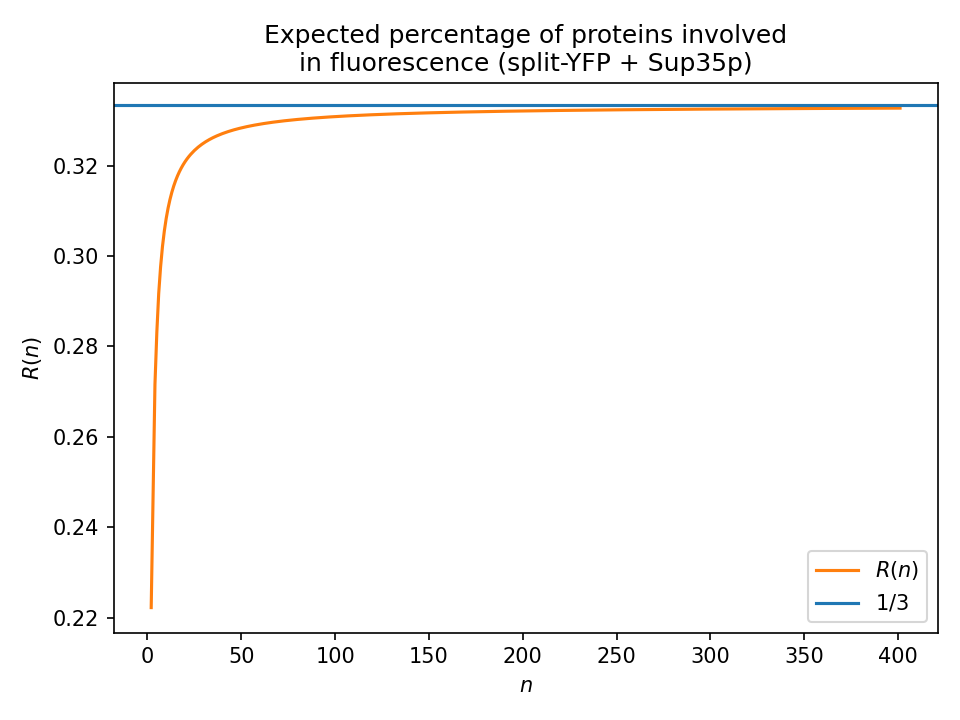
\includegraphics[width=0.75\textwidth]{splityfpandsup35.png}
\caption{$R_{\text{SY}}(n)$ for split-YFP amyloids with Sup35p. The blue line is $1/3$ and the orange curve is the exact $R_{\text{SY}}(n)$. The exponential correction term $O((1/3)^n/n)$ yields even faster convergence than Figure~\ref{fig:splityfp}.}
\label{fig:sup35}
\end{figure}


\section{ Using FRET in amyloids of YFP and CFP}

Consider the case where full YFP (i.e., both halves are conjoined to form the complete fluorophore) and CFP are well-mixed in a container under ambient lighting that causes CFP to fluoresce. When CFP is bonded to YFP, the fluorescence from CFP will cause YFP to fluoresce (FRET). 

We are interested in measuring the \textit{total} yellow fluorescence emanating from amyloids of this kind. That is, the YFPs may fluoresce at a fixed level (call it Level 1) when it is next to one and only one CFP, but it may also fluoresce twice as much (Level 2) if it is next to \textit{two} CFPs as in a YFP being sandwiched between two CFPs. We want to then sum over the total yellow fluorescence of an amyloid rather than just the raw number of YFPs that are caused to fluoresce. We note that this additive model of FRET from multiple donors is a mathematical idealization; in practice, the efficiency of energy transfer from two donors to a single acceptor depends on geometric factors beyond simple adjacency. We adopt this convention for analytical tractability. A more realistic model incorporating geometry-dependent FRET efficiencies would break the linearity-of-expectation argument used below and require a more involved analysis.

Label YFP as Y and CFP as C. Then our patterns are $\{Y,C\}^*$ and as with the split-YFP exclusive case, extracting away the details we get patterns of the form $(0^* 0 1^*1)^* 0^*$, which generates all binary strings of length $n$ beginning with $0$---that is, all $2^{n-1}$ such strings---since there is no blocking constraint on adjacent $1$s in the FRET setting. Here we write a $1$ whenever the full protein at that location causes the previous to fluoresce OR is caused to fluoresce by the previous. We note that, unlike previous cases, once we fix the first protein (Y or C), the 01 pattern uniquely determines every subsequent protein: a $1$ forces the next protein to differ from its predecessor, while a $0$ forces it to match. Therefore, for each 01 pattern there are exactly 2 Y-C sequences (one starting with Y, one with C).

It is now remarked that there is a one-to-one correspondence between 1's as appearing in 0-1 patterns as described above and the total yellow fluorescence emanating from an amyloid of the kind. To be specific, the number of 1's is equal to the total yellow fluorescence (if we take Level 1 to be 1 and Level 2 to be 2 as numerical values for which we sum up). For example:

\begin{alignat}{11}
\text{$\{C, Y \}^*$:  } & C & Y & Y & Y & C & Y & C & Y & Y & C  & C \\
\text{$(0^*0 1^* 1)^* 0^*$:  } & 0 & 1 & 0 & 0 & 1 & 1 & 1 & 1 & 0 & 1 & 0 \\
\text{Yellow fluorescence:  } & 0 & 1 & 0 & 0 & 1 & 2 & 0 & 1 & 1 & 0 & 0
\end{alignat}
Note that in the 01 pattern, each $1$ is attributed to the right endpoint of a $\{C,Y\}$ adjacency as a bookkeeping convention, not to the physically emitting protein. The key claim is that the \textit{total} number of $1$s equals the total yellow fluorescence, which we verify: both rows sum to $6$.

\subsection{Probability of $k$ total yellow fluorescence in length $n$ amyloid}

The number of amyloids of length $n$ with $k$ total yellow fluorescence is:

\[
\cA(n,k) = 2\binom{n-1}{k}, \quad k \in [0,n - 1]
\]

and thus the probability of observing $k$ total yellow fluorescence in a length $n$ amyloid is


\[
P(n,k) = \frac{2\binom{n-1}{k}}{2^n} = \frac{\binom{n-1}{k}}{2^{n-1}}, \quad k \in [0,n - 1]
\].

This is the Binomial$(n-1, 1/2)$ distribution, which can also be seen directly. Let $\varepsilon_i = \pm 1$ according to whether protein $i$ is C or Y, and define $d_i = \varepsilon_i \cdot \varepsilon_{i-1}$ for $i \ge 2$. Then $f_i = 1$ iff $d_i = -1$. The map $(\varepsilon_1, \ldots, \varepsilon_n) \mapsto (\varepsilon_1, d_2, \ldots, d_n)$ is a bijection on $\{\pm 1\}^n$ (since $\varepsilon_i = \varepsilon_1 \prod_{j=2}^i d_j$ is recoverable), so $(d_2, \ldots, d_n)$ are mutually independent and uniform on $\{\pm 1\}$. Hence $f_2, \ldots, f_n$ are mutually independent Bernoulli$(1/2)$ despite their overlapping definition, and their sum is Binomial$(n-1, 1/2)$.

\subsection{Expected total yellow fluorescence}

This is simply the sum:

\[
    E(n) = \sum_{k = 0}^{n - 1} k \cdot P(n,k) 
\]

by definition of expected value.

Note that, by a standard identity \cite[\S 5.1, Eq.~5.5]{gkp1994}:

\begin{align*}
E(n) := \frac{1}{2^{n-1}} \cdot \sum_{k=0}^{n - 1} k \cdot \binom{n-1}{k} 
 =  \frac{1}{2^{n-1}} \cdot (n-1) 2^{n-2} = \frac{n - 1}{2}
\end{align*}

So that for very large $n$, we expect to see about as much yellow unit fluorescence as half the length of the amyloid.

Note that $E(n) = (n-1)/2$ also follows directly from linearity of expectation: the total yellow fluorescence equals the number of adjacent $\{C,Y\}$ pairs, and there are $n - 1$ adjacent pairs each with probability $P(\{C,Y\}) = 2 \cdot (1/2)^2 = 1/2$ of being a $\{C,Y\}$ pair (since FRET interactions, unlike split-YFP fusion, have no blocking constraint). We define the fluorescence ratio as
\[
R_{\text{F}}(n) := E(n)/n = \frac{n-1}{2n} \longrightarrow \frac{1}{2} \text{ as } n \to \infty
\]

The first 400 values of $R_{\text{F}}(n)$ appear in Figure~\ref{fig:fretonly}.

\begin{figure}[ht]
\centering
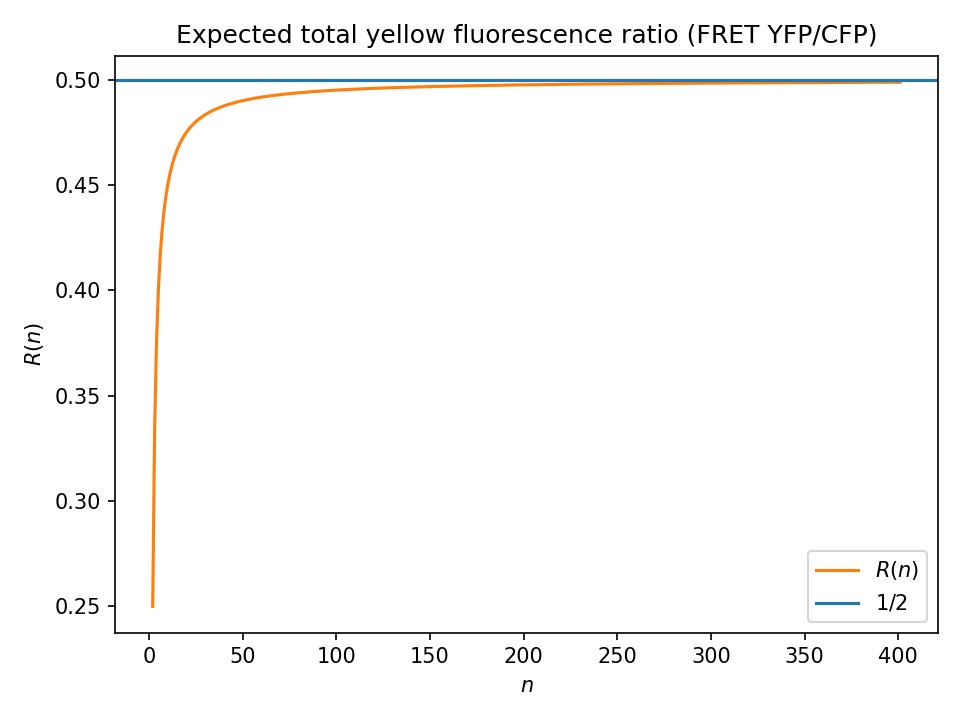
\includegraphics[width=0.75\textwidth]{FretOnly.png}
\caption{$R_{\text{F}}(n)$ for FRET YFP/CFP amyloids. The blue line is $1/2$ and the orange curve is the exact $R_{\text{F}}(n) = (n-1)/(2n)$. Convergence is algebraic ($O(1/n)$), with no exponential correction.}
\label{fig:fretonly}
\end{figure}

\section{Using FRET in amyloids of YFP, CFP, and Sup35p}
As with section 3, we will now analyze the case of introducing Sup35p to the system in Section 4. That is, we have Sup35p, YFP, and CFP well mixed and of equal concentrations in a container under ambient lighting which causes CFP to fluoresce. The cyan fluorescence of a CFP will cause an adjacent YFP to fluoresce yellow due to FRET, and this fluorescence can be stacked so that a YFP sandwiched between two CFPs will fluoresce twice as much as in the case where a YFP is next to only 1 CFP. The presence of Sup35p will block the YFPs and CFPs from interacting under FRET.

Our pattern becomes $\{C,Y,S \}^*$ where $C$ represents CFP, $Y$ represents YFP, and $S$ represents Sup35p. The 01 pattern is still $(0^* 0 1^*1)^* 0^*$ as before. 

\subsection{Probability of $k$ total yellow fluorescence in length $n$ amyloid}

We remark that the number of amyloids of length $n$ with $k$ total yellow unit fluorescence is:


\[
    \cA(n,k) = \sum_{q=0}^{n-k} b_q \sum_{i = 1}^k \sum_{\substack{\sum_{j=1}^i \phi_j = n - q \\ \phi_j \in [2,n-q] \cap \bZ}} \sum_{\substack{\sum_{j=1}^i \psi_j = k \\ \psi_j \in [1, \phi_j] \cap \bZ}} \prod_{j=1}^i a_{\phi_j,\psi_j}
\]

where 

\begin{align*}
b_0 &= 1, \\
b_1 &= 3, \\
b_i &= 2b_{i-1} + b_{i-2} \text{ for } i > 1,
\end{align*}

and 

\begin{align*}
a_{n,y} &= 0, \text{ for } n < y + 1 \\
a_{y+1,y} &= 2\\
a_{y+2,y} &= 2\\
a_{n,y} &= 2a_{n-1,y} + a_{n-2,y}, \text{ for } n > y + 2
\end{align*}

Explicitly,

\[
b_n = - \frac{1}{2 + 2\sqrt{2}} \cdot \left(\frac{1}{-1-\sqrt{2}}\right)^n - \frac{1}{2-2\sqrt{2}} \cdot \left( \frac{1}{-1 +\sqrt{2}} \right)^n, n \ge 0 
\]

which is the same $b_n$ in section 3, and

\[
a_{n,y} =
\begin{cases}
      0, \text{if} \  n \le y \\
      -\frac{4+3\sqrt{2}}{2+\sqrt{2}} \left( \frac{1}{-1-\sqrt{2}}  \right)^{n-y}   + \frac{4-3\sqrt{2}}{2-\sqrt{2}} \left(\frac{1}{-1 + \sqrt{2}} \right)^{n-y}, \text{if} \ n > y \\ 
\end{cases}
\]

We now derive these formulas.

As before in Section 3, the argument is to let $b_q$ represent the tail of zeros of length $q$ (which corresponds to the tail $0^*$ in our functional regular expression), $i$ the number of blocks of the form $(0^* 0 1^* 1)$ (as per our functional regular expression), $\phi_j$ is the length of the $j$th block of the form  $(0^* 0 1^* 1)$ , $\psi_j$ is the number of $1$'s in the $j$th block of the form $(0^* 0 1^* 1)$, and $a_{x,y}$ is the total number of $C-Y-S$ patterns corresponding to a 01 block of the form $(0^* 0 1^* 1)$ of length $x$ and with $y$ 1's. The formula then follows by the same decomposition used for $\cA(n,k)$ in Section 3.

We now justify the recurrences.

For $b_i$, note that it represents the number of C-Y-S patterns represented by a 0-1 pattern of the form 000...0 where there are precisely $i$ 0's. To obtain the recursive formula, we note that the C-Y-S patterns of this type are represented by the C-Y-S regular expression
\[
S^* \{CC^* SS^*, YY^* SS^*\}^* \{CC^*, YY^*, \varepsilon\}
\]
where $\varepsilon$ denotes the empty string.
Notice that this is the same as in Section 3 where $b_i$ represented the number of A-B-S patterns represented by a 0-1 pattern of the form 000...0 where there are precisely $i$ 0's -- the regular expression is equivalent by replacing C with A and Y with B. Thus, this is why we get the same formula for $b_i$ here as we did in Section 3 and do not need to show any new details.

As for $a_{n,y}$, consider that it represents the number of C-Y-S patterns corresponding to a 0-1 functional pattern of length $n$ and with $y$ 1's, and looks like 00000...00011111...111. We fix $y = j$. Then for each $n \in \bN$, a regular expression is as follows:

\[
S^* \{CC^* SS^*, YY^* SS^*\}^* \{C(YCY...), Y(CYC...) \}
\]

where for the last term the patterns C(YCY...) or Y(CYC...) are of length $j + 1$.

Our generating function is thus:


\[
G(x) = \sum_{i=0}^\infty a_{i,j} x^i = \frac{1}{1-S} \cdot \frac{1}{1 - \left(\frac{C}{1-C} \cdot \frac{S}{1-S} + \frac{Y}{1-Y} \cdot \frac{S}{1-S} \right)} \cdot 2x^{j+1}
\].

Setting $C = Y = S = x$, this simplifies to

\[
G(x) = \frac{2x^{j+1}(1-x)}{1-2x-x^2}
\]

and so

\[
a_{n,j} - 2a_{n - 1,j} - a_{n-2,j} = 
\begin{cases}
      0, & \text{if}\ n < j + 1 \\
      2, & \text{if}\ n= j + 1 \\
      -2, & \text{if}\ n= j + 2 \\
        0, & \text{if} \ n > j + 2  
    \end{cases}
\]

where the recurrence is read off from the generating function as before.

To get the explicit formula, note that we cannot do partial fractions on $G(x)$ directly, however we can notice that the values of $a_{n,y}$ is simply a translation in the positive direction along $\bR$ of the values $a_{n,0}$ in its first index by $y$ -- the second index. That is, given that the recursive formula is:
\begin{align*}
a_{n,y} &= 0, \text{ for } n < y + 1 \\
a_{y+1,y} &= 2\\
a_{y+2,y} &= 2\\
a_{n,y} &= 2a_{n-1,y} + a_{n-2,y}, \text{ for } n > y + 2,
\end{align*}
one should notice that $y$ determines when the sequence formally starts to have non-zero values and thus becomes non-trivial. With that in regard, $a_{n,y}$ is essentially a class of sequences in terms of $y$ which all have essentially the same sequence of values for all $n \in \bN$, modulo the zeroes at the beginning. Hence the notion of the second index $y$ being a "translation" factor. The translation rule is formally
\[a_{n,j} = a_{n+\ell,\, j-\ell}
\]
for any integer $\ell$ such that both indices remain in range.
With this in mind, consider that we have the generating function in terms of $j$ which is the second index. Setting $j = 0$ gives a generating function for $a_{n,0}$ which we can do partial fractions on:

\begin{align*}
    G(x) &= \frac{2x(1-x)}{1-2x-x^2} = 2 + \frac{6x-2}{1-2x-x^2} = 2 +  \frac{(4+ 3\sqrt{2})/\sqrt{2}}{(-1-\sqrt{2}) - x} - \frac{(4-3\sqrt{2})/\sqrt{2}}{(-1+\sqrt{2}) - x} \\
    &=2  - \frac{4+3\sqrt{2}}{2+\sqrt{2}} \cdot \frac{1}{1-\frac{1}{-1-\sqrt{2}} x} + \frac{4-3\sqrt{2}}{2-\sqrt{2}} \cdot \frac{1}{1- \frac{1}{-1+\sqrt{2}}x} \\
    &= 2  - \frac{4+3\sqrt{2}}{2+\sqrt{2}}  \sum_{i=0}^\infty \left( \frac{1}{-1-\sqrt{2}}  \right)^i x^i  + \frac{4-3\sqrt{2}}{2- \sqrt{2}} \sum_{i=0}^\infty \left(\frac{1}{-1+\sqrt{2}} \right)^i x^i
\end{align*}

Hence we get that 
\[
a_{n,0} = 
\begin{cases}
      0, \text{if} \  n \le 0 \\
      -\frac{4+3\sqrt{2}}{2+\sqrt{2}} \left( \frac{1}{-1-\sqrt{2}}  \right)^n   + \frac{4-3\sqrt{2}}{2-\sqrt{2}} \left(\frac{1}{-1 + \sqrt{2}} \right)^n, \text{if} \ n > 0 \\ 
\end{cases}
\]

Hence by the translation rule,

\[
a_{n,y} =
\begin{cases}
      0, \text{if} \  n \le y \\
      -\frac{4+3\sqrt{2}}{2+\sqrt{2}} \left( \frac{1}{-1-\sqrt{2}}  \right)^{n-y}   + \frac{4-3\sqrt{2}}{2-\sqrt{2}} \left(\frac{1}{-1 + \sqrt{2}} \right)^{n-y}, \text{if} \ n > y \\ 
\end{cases}
\]
which is what was required.

\textbf{Verification.} For $n = 3$, brute-force enumeration over all $3^3 = 27$ amyloids in $\{C,Y,S\}^3$ gives $\cA(3,0) = 17$, $\cA(3,1) = 8$, and $\cA(3,2) = 2$, with $E(3) = (0 \cdot 17 + 1 \cdot 8 + 2 \cdot 2)/27 = 12/27 = 4/9$. This agrees with the linearity-of-expectation formula $E(3) = 2(3-1)/9 = 4/9$.

The combinatorial formula for $\cA(n,k)$ above gives the full probability distribution. However, for computing the expected value, a much simpler route is available. As in Section 4, the total yellow fluorescence of an amyloid equals the number of adjacent $\{C,Y\}$ pairs. Since FRET interactions have no blocking constraint (unlike split-YFP fusion), the linearity of expectation argument from Section 4 applies directly. With each protein independently C, Y, or S with probability $1/3$:
\[
E(n) = (n-1) \cdot P(\{C,Y\} \text{ pair}) = (n-1) \cdot 2 \cdot \frac{1}{3} \cdot \frac{1}{3} = \frac{2(n-1)}{9}
\]

Therefore
\[
R_{\text{F}}(n) := E(n)/n = \frac{2(n-1)}{9n} \longrightarrow \frac{2}{9} \text{ as } n \to \infty
\]

The first 400 values of $R_{\text{F}}(n)$ appear in Figure~\ref{fig:fretsup35}.

\begin{figure}[ht]
\centering

\includegraphics[width=0.75\textwidth]{FretandSup35.png}
\caption{$R_{\text{F}}(n)$ for FRET YFP/CFP amyloids with Sup35p. The blue line is $2/9$ and the orange curve is the exact $R_{\text{F}}(n) = 2(n-1)/(9n)$. Convergence is algebraic ($O(1/n)$), as in Figure~\ref{fig:fretonly}.}
\label{fig:fretsup35}
\end{figure}

\section{Generalization to unequal concentrations}

The results of Sections 2--5 all depend on the equal-concentration assumption. The Markov chain arguments generalize readily to unequal concentrations, which we outline here.

\subsection{Split-YFP with unequal concentrations}
Suppose protein A appears with probability $\alpha$ and protein B with probability $1 - \alpha$. Let $\pi_n$ denote the probability that the $n$th protein is in the unfused state. The transition probabilities are: from unfused, the next protein is the same type with probability $\alpha^2 + (1-\alpha)^2$ (staying unfused) or a different type with probability $2\alpha(1-\alpha)$ (fusion occurs, next protein is fused). From the fused state, the next protein is always unfused. The recurrence is therefore
\[
\pi_{n+1} = \bigl[\alpha^2 + (1-\alpha)^2\bigr]\,\pi_n + (1 - \pi_n)
\]
with fixed point $\pi^* = 1/\bigl(1 + 2\alpha(1-\alpha)\bigr)$. The expected fluorescence contributed by the $(n+1)$th protein is $2\alpha(1-\alpha)\,\pi_n$, so since $R_{\text{SY}}(n) = 2E(n)/n$, at steady state:
\[
\lim_{n \to \infty} R_{\text{SY}}(n) = 2 \cdot 2\alpha(1-\alpha) \cdot \pi^* = \frac{4\alpha(1-\alpha)}{1 + 2\alpha(1-\alpha)}
\]
which reduces to $4 \cdot \frac{1}{4} / \frac{3}{2} = 2/3$ when $\alpha = 1/2$. By symmetry and concavity of $\alpha(1-\alpha)$, this limit is maximized at $\alpha = 1/2$, confirming that equal concentrations maximize the fluorescence yield.

\subsection{Split-YFP with Sup35p at unequal concentrations}
Now suppose proteins A, B, S appear with probabilities $\alpha$, $\beta$, and $1 - \alpha - \beta$ respectively. We define three Markov states: $p_A$ (rightmost is A, unfused), $p_B$ (rightmost is B, unfused), and $q$ (rightmost is S, or fused). The transitions are:
\begin{itemize}
\item From $p_A$: next is A (prob $\alpha$, stay $p_A$), B (prob $\beta$, fuse, go $q$), or S (prob $1{-}\alpha{-}\beta$, go $q$).
\item From $p_B$: next is B (prob $\beta$, stay $p_B$), A (prob $\alpha$, fuse, go $q$), or S (prob $1{-}\alpha{-}\beta$, go $q$).
\item From $q$: next is A (prob $\alpha$, go $p_A$), B (prob $\beta$, go $p_B$), or S (prob $1{-}\alpha{-}\beta$, stay $q$).
\end{itemize}
Solving the balance equations $\pi_A = \alpha\pi_A + \alpha\pi_q$, $\pi_B = \beta\pi_B + \beta\pi_q$, and $\pi_A + \pi_B + \pi_q = 1$ gives $\pi_A = \alpha(1-\beta)/(1 - \alpha\beta)$, $\pi_B = \beta(1-\alpha)/(1 - \alpha\beta)$, and $\pi_q = (1-\alpha)(1-\beta)/(1-\alpha\beta)$. The expected fluorescence per step is $e = \beta\pi_A + \alpha\pi_B = \alpha\beta(2 - \alpha - \beta)/(1 - \alpha\beta)$, giving
\[
\lim_{n \to \infty} R_{\text{SY}}(n) = 2e = \frac{2\alpha\beta(2 - \alpha - \beta)}{1 - \alpha\beta}
\]
which reduces to $1/3$ when $\alpha = \beta = 1/3$ (and to $2/3$ when $\alpha = \beta = 1/2$, recovering the no-Sup35p case).

\subsection{FRET with unequal concentrations}
In the FRET setting with $P(C) = p_C$, $P(Y) = p_Y = 1 - p_C$, linearity of expectation gives $R_{\text{F}}(n) \to 2p_C p_Y$ directly, and with Sup35p at concentration $p_S$ (where $p_C + p_Y + p_S = 1$) the limit is likewise $R_{\text{F}}(n) \to 2p_C p_Y$. These generalizations would allow the model to be calibrated to experimental concentration ratios.

\section{Conclusion}

We have derived exact probability distributions and closed-form expected values for fluorescence in four combinatorial models of amyloid fibrils. The principal results are summarized in the following table:

\begin{center}
\begin{tabular}{lcccc}
\hline
System & Ratio & Exact $E(n)$ & Exact ratio & Limit \\
\hline
Split-YFP (Sec.~2) & $R_{\text{SY}} = \dfrac{2E}{n}$ & $\dfrac{3n-2}{9} + \dfrac{2(-1)^n}{9 \cdot 2^n}$ & $\dfrac{2(3n-2)}{9n} + \dfrac{2(-1)^n}{9n \cdot 2^{n-1}}$ & $2/3$ \\[8pt]
Split-YFP + Sup35p (Sec.~3) & $R_{\text{SY}} = \dfrac{2E}{n}$ & $\dfrac{4n-3}{24} - \dfrac{(-1)^{n-1}}{24 \cdot 3^{n-1}}$ & $\dfrac{4n-3}{12n} + \dfrac{(-1)^n}{12n \cdot 3^{n-1}}$ & $1/3$ \\[8pt]
FRET YFP/CFP (Sec.~4) & $R_{\text{F}} = \dfrac{E}{n}$ & $\dfrac{n-1}{2}$ & $\dfrac{n-1}{2n}$ & $1/2$ \\[8pt]
FRET + Sup35p (Sec.~5) & $R_{\text{F}} = \dfrac{E}{n}$ & $\dfrac{2(n-1)}{9}$ & $\dfrac{2(n-1)}{9n}$ & $2/9$ \\[4pt]
\hline
\end{tabular}
\end{center}
\noindent Here $R_{\text{SY}}(n) := 2E(n)/n$ is the fraction of proteins participating in split-YFP fluorescence (two proteins per fused pair), while $R_{\text{F}}(n) := E(n)/n$ is total FRET fluorescence per protein. The two ratios measure different physical quantities and are not directly comparable.

A key structural distinction separates the two pairs of systems. In the split-YFP settings (Sections 2 and 3), the adjacency blocking constraint---a fused pair cannot participate in further fusion---introduces nontrivial combinatorial structure. This necessitates generating function techniques to derive the full distributions $P(n,k)$ and Markov chain arguments to compute the expected values in closed form. The agreement between these two independent approaches provides mutual verification of both the sum identities and the Markov chain analysis.

In the FRET settings (Sections 4 and 5), the absence of a blocking constraint means that each adjacent pair contributes independently to the total fluorescence. This permits a direct linearity-of-expectation argument, yielding exact formulas without the need for the full combinatorial machinery.

The limiting ratios have concrete experimental interpretations. For split-YFP amyloids, $R_{\text{SY}}(n) \to 2/3$ means that in a long amyloid composed of equal concentrations of the two halves, approximately two-thirds of the proteins participate in a fluorescent fusion---a high baseline fluorescence yield arising from the alternating tendency of random binary sequences. Introducing Sup35p at equal concentration halves this to $1/3$: the inert Sup35p proteins act as spacers that interrupt potential fusion pairs. For FRET, the ratio $R_{\text{F}}(n) \to 1/2$ reflects the probability that a random adjacent pair is a $\{C,Y\}$ pair, while the drop to $2/9$ with Sup35p reflects the reduced probability $2 \cdot (1/3)^2$ of such a pair when three protein types compete for each position. Experimentally, measured fluorescence ratios deviating from these baseline values would indicate non-random assembly biases in the amyloid growth process.

A natural extension of the FRET model would be to allow interactions within a window of radius $r$ rather than nearest neighbors only. For $r = 2$, a YFP at position $i$ would fluoresce from CFPs at positions $i \pm 1$ and $i \pm 2$. The indicator variables $f_i$ are then no longer independent---knowing that positions $i-1$ and $i$ are a $\{C,Y\}$ pair constrains the distribution at $i+1$---and the linearity-of-expectation argument no longer suffices for the full distribution $P(n,k)$. One would need either inclusion-exclusion or a Markov chain with states tracking the last $r$ proteins. For the expected value $E(n)$, linearity of expectation still applies: each pair $(i, j)$ with $|i - j| \le r$ contributes to $E(n)$ by linearity of expectation (the indicators are correlated but linearity does not require independence), giving $E(n) = \sum_{d=1}^{r} (n - d) \cdot 2p_C p_Y$ for the FRET + Sup35p case with equal concentrations. However, the full distribution would require generating functions for strings with forbidden patterns of length $> 2$, a substantially richer combinatorial problem.

Our analysis assumes that proteins are independently distributed in the amyloid sequence. This assumption neglects known cooperative and templated growth effects in amyloid assembly \cite{chiti2006} and should be interpreted as a combinatorial null model: a baseline against which experimental deviations---reflecting assembly biases, kinetic trapping, or cooperative interactions---could be quantified. The combinatorial framework developed here, particularly the generating function approach to constrained fluorescence patterns via regular expressions, could in principle be adapted to non-uniform protein distributions if experimental data on assembly biases become available.

All simulation and verification scripts referenced in this paper (\texttt{split\_yfp\_simulation.py}, \texttt{sup35\_simulation.py}, \texttt{fret\_sup35\_simulation.py}, and associated plotting scripts) are available at \url{https://github.com/danielchen0/amyloids}.

\bibliographystyle{plain}
\bibliography{references}
\end{document}
